\capitulo{5}{Aspectos relevantes del desarrollo del proyecto}

En este apartado se pretende resumir los aspectos más relevantes que se han tratado y cómo se han resuelto las diferentes dificultades encontradas a lo largo de su desarrollo.



\section{Dificultades encontradas en el desarrollo}

Este proyecto se ha caracterizado por las diversas dificultades que se han encontrado primordialmente exacerbadas por las incompatibilidades de diversas librerías y herramientas en el desarrollo móvil.
A continuación, describo alguno de los problemas más significativos y cómo los he abordado.

\subsection{Incompatibilidad con biblioteca Web3}

En el momento en el que se intentó realizar la primera conexión con el contrato desde la aplicación móvil, surgió un problema con la biblioteca Web3, esencial para la interacción entre el frontend y el contrato inteligente.
El error se producía a la hora de ejecutar la aplicación de forma nativa en el dispositivo móvil.
El error describía un problema 'ReferenceError' indicando que la propiedad `EventTarget' no existía en el motor de JavaScript Hermes utilizado por React Native. 

\texttt{ReferenceError: Property `EventTarget' doesn't exist, js engine: hermes ERROR Invariant Violation: `main' has not been registered.}

Sin embargo, desplegando la aplicación en un entorno web desde el navegador de mi ordenador esta biblioteca no producía ningún error y se consiguió establecer conexión exitosamente con el contrato inteligente.
Este fue un problema que se alargó durante los dos siguientes \textit{sprints} y se investigó de forma reiterada. Temiendo que se debía a un error de incompatibilidad con las versiones de las bibliotecas en mi proyecto, se fue probando diferentes combinaciones hasta que usando la versión 4.1 de la biblioteca Web3 ese error desapareció.
El problema no se había solucionado ya que dicho error solo desapareció dejando paso a un nuevo error, en este caso el error describía un problema de reconocimiento similar al anterior pero con la propiedad 'TextEncoder' la cual es parte de la API de codificación que proporciona una forma de codificar texto en varios formatos, comúnmente utilizados en entornos web.

\texttt{ReferenceError: Property `TextEncoder' doesn't exist, js engine: hermes.}

React native no implementa todas las API web estándar que se encuentran en los navegadores modernos, por lo que es necesario agregar dicha característica de forma manual. Para ello he hecho uso de un \textit{polyfill}, que es una biblioteca que pretente proporcionar una implmentación alternativa a la API de funciones nativas.
Por tanto, se ha instalado `text-encoding', que es un polyfill para la API de `TextEncoder'.
Seguidamente se ha creado un nuevo archivo en la raíz del proyecto al que he llamado `globals.js', en este archivo se ha asignado `TextEncoder' de `text-encoding' a `global.TextEncoder'. Es decir, que he agregado 'TextEnoder' al objeto global `global' que actúa de forma similar al objeto `window' en los navegadores.

\texttt{global.TextEncoder = require(`text-encoding').TextEncoder;}

Luego importando `globals.js' en mi archivo `App.js' aseguro que `TextEncoder' este disponible globalmente antes que cualquier otro objeto que dependa de él, evitando errores de referencia.


\subsection{Tamaño de contrato muy grande}

Durante el desarrollo en Solidity del contrato inteligente surgió un desafío inesperado relacionado con el tamaño del código del contrato.
El proceso de desarrollo del contrato inteligente se ha realizado de forma iterativa, empezando con funciones básicas y gradualmente se fue implementando funcionalidades más complejas. Después de cada adición significativa, se procedía a migrar y testear el contrato para asegurar su correcto funcionamiento y rendimiento.

En una de estas iteraciones, al intentar migrar el contrato, apareció un error que exponía un problema de que el código había superado los 24576 bytes de tamaño, un límite establecido por la actualización "Spurious Dragon" de Ethereum. Este límite fue introducido para mitigar riesgos de ataques de denegación de servicio (DoS) que podrían ocurrir si se permitiera desplegar contratos de tamaño excesivamente grande.

\textit{code size is 26466 bytes and exceeds 24576 bytes (a limit introduced in Spurious Dragon). This contract may not be deployable on Mainnet. Consider enabling the optimizer (with a low "runs" value!), turning off revert strings, or using libraries.}

Con el objetivo de que el contrato sea menor de esos 24576 bytes y así mantener toda la funcionalidad en un único contrato facilitando así su gestión y uso, se aplicaron diversas técnicas.
En una primera instancia, se hizo una revisión del código para identificar y eliminar redundancias, optimizar las funciones existentes, y donde fue posible, integrar librerías externas que reemplazaran bloques de código repetitivos.
Por otro lado, se habilitó el optimizador del compilador de Solidity, ajustando el número de \textit{runs} a un valor bajo, con la intención de reducir significativamente el tamaño del bytecode generado al optimizar la compilación con base en la frecuencia esperada de ejecución del código.

Sin embargo, a medida que el proyecto evolucionaba y con la aparición de nuevas funcionalidades para implementar, esta estrategia de optimización dejó de ser sostenible y fue necesario modularizar el código. 
Para ello se dividió el contrato en múltiples contratos más pequeños que interactúen entre sí mediante herencia o mediante llamadas a funciones de otros contratos.
La modularización no solo ayudó a gestionar mejor el tamaño del contrato, sino que también mejoró la mantenibilidad y la actualización del código.



\subsection{Problemas implementación MetaMask}

La integración de una billetera de terceros en el proyecto ha presentado un gran desafío, con la idea de implementar una solución que permitiera al usuario gestionar sus cuentas, se exploraron diferentes posibilidades.
En este caso, se optó por la opción implementar MetaMask, debido a ser la billetera ampliamente más conocida y usada por la comunidad. 
Por lo tanto, la idea era usar los servicios de MetaMask para que los usuarios pudieran acceder a la aplicación móvil con su cuenta personal y más adelante poder interactuar con dicha cuenta.

Inicialmente, se hicieron diferentes pruebas para establecer una conexión entre MetaMask y mi aplicación. Estas pruebas se centraron en utilizar la extensión de navegador de MetaMask con el objetivo de establecer la conexión, donde se consiguió establecer una conexión estable y continua permitiendo interactuar con la billetera libremente. Aunque esta implementación solo aseguraba el funcionamiento de la aplicación en un entorno de navegador.

Partiendo de su correcto funcionamiento en navegador se quiso expandir la funcionalidad para que fuera compatible en la aplicación móvil.
Este paso resultó ser considerablemente más complejo debido a la incompatibilidad directa de las extensiones de navegador en los entornos móviles. 
Inicialmente se intentó usar el SDK de MetaMask, recientemente lanzado, empleando un enfoque de enlaces profundos para interacción directa con la aplicación de MetaMask en dispositivos móviles.
La idea era, que una vez el usuario hubiera configurado correctamente sus cuentas en la app de Metamask, cuando quisiera realizar alguna operación que requeriese de la billetera, la aplicación móvil generaría un URI de MetaMask que abriría directamente la aplicación de MetaMask instalada en el dispositivo del usuario. Desde allí el usuario podría autorizar la operación.
No obstante, este método enfrentó grandes obstáculos técnicos, impidiendo establecer una conexión con la aplicación móvil de MetaMask.

A raíz de este problema se investigaron alternativas para poder ofrecer una conexión estable entre la aplicación y la billetera móvil. De esta forma se planteó la utilización de 'WalletConnect', un protocolo de código abierto altamente utilizado por la comunidad y que facilita la comunicación entre billeteras móviles y aplicaciones descentralizadas mediante enlaces seguros. Tras un largo proceso de desarrollo, se logró implementar WalletConnect con la posibilidad de establecer conexiones no solo con MetaMask sino con otras cientos de billeteras.

Sin embargo, la aplicación aún no era capaz de realizar operaciones a través de esta nueva configuración. Durante un par de \textit{sprints} dedicados principalmente a este problema, se identificó la necesidad de una revisión completa de la arquitectura de la aplicación. 
Para ello se abandonó la biblioteca Web3, que había sido la pieza fundamental de conexión entre los contratos inteligentes y el frontEnd.
En su lugar, se adaptó la aplicación para usar las bibliotecas Ethers, Wagmi y Viem, que ofrecían una mayor flexibilidad y compatibilidad con WalletConnect.

Esto proceso fue bastante tedioso ya que implicó establecer una nueva conexión con el contrato mediante el nuevo provedor, así como actualizar todas las llamadas al contrato inteligente para que estas puedan ser ejecutadas correctamente por la billetera configurada en WalletConnect.
Esta transformación no solo resolvió los problemas iniciales, sino que también se mejoró la accesibilidad de la aplicación permitiendo la integración de cientos de billeteras.



\subsection{Incompatibilidad con Ganache y Metamask}

Entre los problemas que han surgido debido a incompatibilidades con la aplicación móvil, se ha identificado un error el cual imposibilita crear y conectar una red Ganache desde la aplicación móvil de MetaMask. Al igual que sucedía con la biblioteca Web3, este problema no existe en el desarrollo web.

Como he mencionado anteriormente, para la ejecución de mi proyecto es necesario desplegar una red Ganache la cual normalmente se despliega en \textit{localhost}. Sin embrago, para que el resto de dispositivos de la red puedan interactuar con ella, es neceario asignarle una dirección IP específica, en este caso la dirección IP de mi ordenador.
Al desplegar Ganache se muestran datos importantes como la URL RPC y la ID de la cadena, las cuales son esenciales para configurar una red personaliada en MetaMask.
A partir de esta configuración, Metamask permite importar cuentas disponibles en el entorno local de Ganache a través de su clave privada, replicando de esta forma un uso realista en el entorno de prueba de como se realizarían las interacciones mediante la billetera, la cual funciona como interfaz para interactuar con la blockchain.

Sin embargo, he encontrado un problema al realizar este proceso en la aplicación móvil de MetaMask, a diferencia de la extensión de nevagador, la aplicación móvil no soporta de manera uniforme las redes HTTP Y HTTPS, devolviendome el siguiente error:

\texttt{Could not fetch chain ID. Is your RPC URL correct?}

Este mensaje indica que no se puede recuperar el ID de la cadena, el cual es un identificador único de cada blockchain, crucial para la seguridad, utilizado por las billeteras para asegurar que interactúan con la red correcta.
Este problema radica en que comúnmente, Ganache despliega la red usando HTTP en un entorno local, lo cual es apto para la extensión de navegador, pero no para la aplicación móvil ya que requiere HTTPS.
Este es un problema recurrente para muchos desarrolladores y aún no cuenta con una solución directa. Una solución temporal es crear un túnel seguro y exponer la red Ganache local usando herramientas como ngrok, que proporciona una URL HTTPS temporal. De esta forma se expone un servidor local a internet a través de un túnel seguro, permitiendo así que la aplicación de MetaMask establezca una conexión segura.
Bien es cierto, que esto soluciona en cierta parte el problema, pero es solo una solución temporal y no es ideal para entornos de producción.


\subsection{Desafíos del despliegue en Mainnet}

Dada la imposibilidad de utilizar Ganache en conjunto con MetaMask,se hizo necesario a buscar una solución al problema para poder integrar una billetera en el proyecto.
En el proceso de investigación para resolver este problema, se dedujo que la única opción para poder usar MetaMask era desplegar el contrato en una red blockchain real.

Para poder integrar MetaMask en el proyecto y realizar operaciones sin que suponga ningún coste económico real, se decidió usar la red de Sepolia, que es una red de prueba de Ethereum. 
Esta idea, finalmente acabó complicando el proyecto notablemente, siendo necesaria una adaptación de todo el código que llevó varías semanas de trabajo.
Para usar la red de Sepolia, fue necesario desplegar el contrato en dicha red. El primer paso fue obtener ETH de Sepolia, necesarios para cubrir los costes del despliegue, lo cual es un proceso lento debido a las pequeña cantidad que se puede obtener diariamente. 
Además, para interactuar con una red real, fue esencial establecer un proveedor de servicios de terceros. Para esta tarea se seleccionó Infura. La cual mediante una URL permite interactuar con la red Ethereum sin la necesidad de ejecutar un nodo de Ethereum propio. 

Seguidamente fue necesario llevar a cabo la configuración de Truffle para poder desplegar el contrato en esta red, haciendo uso de la URL proporcionado por Infura y de una cuenta Ethereum con suficientes fondos.
Una vez desplegado el contrato, es necesario establecer conexión con el contrato desde la aplicación, proceso que también se hace mediante los servicios de Infura.
Para este paso, debido a las grandes dificultades 
A pesar de los múltiples problemas enfrentados con la biblioteca Web3 durante todo el desarrollo, y debido a la incompatibilidad con WalletConnect, para este paso se decidió utilizar la biblioteca Ethers, que proporcionó una integración más fluida y estable.

Por otro lado, para el correcto funcionamiento de la aplicación en una red blockchain real, fue necesario modificar todo el código donde se realizase alguna operación sobre el contrato.
Una vez configurado todo, y en combinación con WalletConnect, se realizaron las primeras operaciones. Sin embargo, los tiempos de espera para la confirmación de acciones y las operaciones de lectura se vieron significativamente afectados por la latencia de la red principal, lo cual requirió de ajustes adicionales en la aplicación para mejorar la fluidez y la experiencia del usuario.

A pesar de los éxitos iniciales, surgieron problemas al desplegar el contrato inteligente nuevamente en la red Sepolia, la API de Infura reportó que se había superado el límite de llamadas. 
Este fue un problema inesperado, debido que hasta el momento se había logrado desplegar el contrato en varias ocasiones. 
No puedo asegurar el origen del problema, pero seguramente tenga que ver con que días antes la empresa reportó una alta demanda y se realizaron limitaciones en los servicios de IPFS. 
Hasta día de hoy la API sigue devolviendo dicho error, por lo que esto llevó a explorar alternativas como Alchemy, que ofrecía límites más generosos en sus consultas. 
A pesar de lograr desplegar el contrato usando Alchemy, se encontraron dificultades para interactuar desde la aplicación con el contrato a través de este proveedor.

Ante la acumulación de desafíos y la falta de tiempo, se tomó la decisión de regresar a la implementación inicial utilizando Ganache, lo que resultó en una aplicación más estable y manejable para la detección de errores, pero sin la posibilidad de implementar el inicio de sesión con una billetera. Este cambio, aunque marcó un retroceso en a etapas anteriores del diseño e implementación de la aplicación, permitió un contacto valioso con la red Ethereum real y abrió caminos para el futuro desarrollo del proyecto, dejando establecida una base de código preparada para operar en este entorno.



\section{Incompatibilidad Firebase}

Durante la fase inicial del proyecto se optó por implementar una base de datos para la autenticación de los usuarios.
Se decidió usar Firebase, debido a que es una herramienta muy poderosa y robusta, y mi interés de aprender a utilizarla. Entre las funcionalidades previstas estaban la autenticación de usuarios, el almacenamiento de datos y un servicio sólido de mensajería para funciones como el restablecimiento de contraseña y la verificación de dos factores.
Además, se contempló la posibilidad de permitir iniciar sesión con google, una funcinalidad nativa de esta base de datos.

En una primera instancia se implementó correctamente las funcionalidades de registro, verificación y recuperación de contraseña.
Sin embargo, en el momento que se importaba la biblioteca de Web3, la aplicación compilaba sin errores, pero el proceso de autenticación de usuarios fallaba, retornando un error sin una solución clara tras varias investigaciones.

A medida que el proyecto evolucionaba, surgió la idea de establecer un inicio de sesión usando billeteras como MetaMask y más adelante WalletConnect. Considerando esta integración, mantener la autenticación de Firebase parecía redundante, por lo que se decidió prescindir de la idea de realizar la autenticación de usuario con firebase en favor de la autenticación basada en billeteras.
 
No obstante, en las últimas semanas de desarrollo del proyecto como bien se ha comentado anterioridad, tras enfrentar múltiples dificultades con la implementación de las billeteras y descartar dicha posibilidad, la necesidad de implementar una autenticación de usuario resurgió.
Por lo tanto, se reanudó la investigación sobre la incompatibilidad de Firebase y la biblioteca Web3, debido a un error específico que se desencadenaba por la presencia de Web3 en el proyecto, afectando la verificación de usuarios.

Tras un análisis y varias pruebas, se ideó una solución que consistía en implementar la importación `perezosa' de Web3 (ver imagen \ref{img:CodeWeb3Lazy}). Esto implica cargar Web3 sólo después de que la autenticación de usuario fuera exitosa. Para llevar a cabo esta estrategia, se utilizó la técnica de `dynamic imports' de JavaScript, que permite cargar módulos de manera condicional y asíncrona. 
Para ello, en vez de importar la biblioteca Web3, se llamará a este fragmento de código, el cual primero verifica si ya existe una instancia de Web3, devolviendo esta instancia si está disponible. En caso de que no haya una instancia previa, se procede a importar Web3 de manera dinámica solo cuando el usuario necesite realizar una acción que involucre dicha biblioteca.
Además, el uso de promesas asegura que la carga del módulo se maneje de manera asíncrona  sin interrumpir la interacción del usuario.

\begin{figure}[h]
	\label{img:CodeWeb3Lazy}
	\centering
	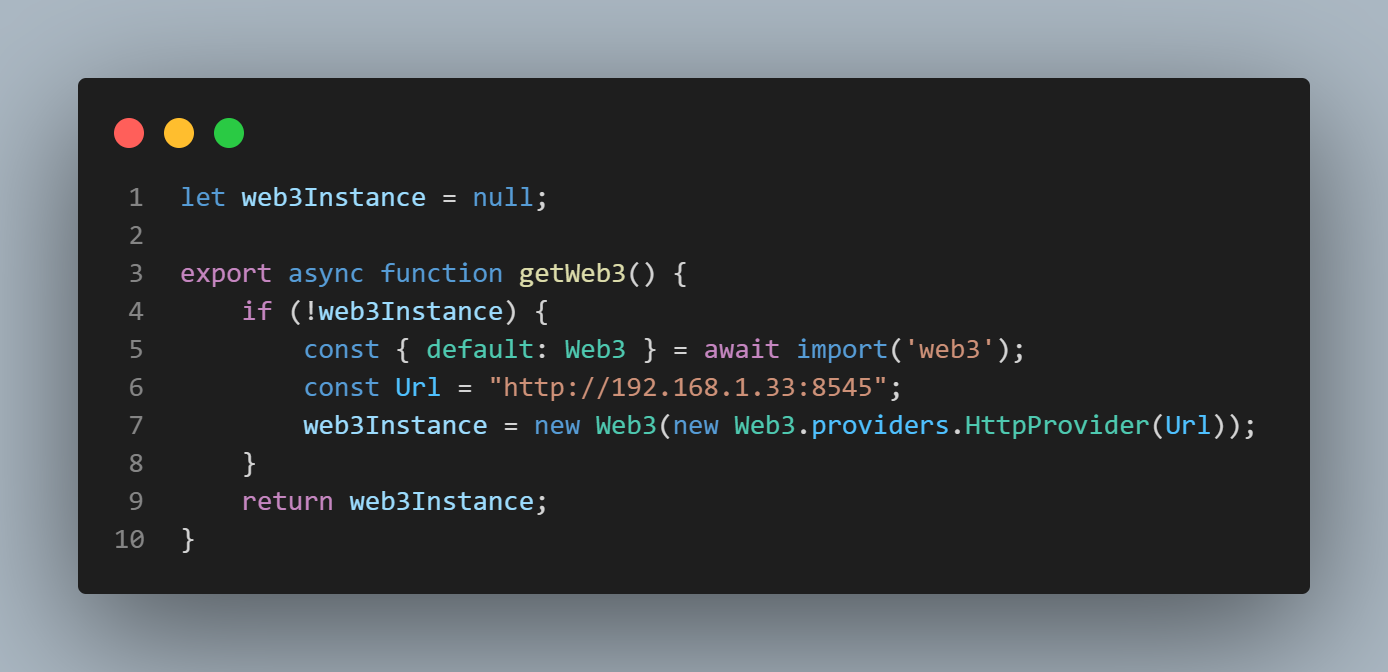
\includegraphics[width=\textwidth]{CodeWeb3Lazy}
	\caption[Importación perezosa Web3]{Importación perezosa Web3.}
\end{figure}

Este ajuste no sólo resolvió el problema técnico, sino que también permitió mantener el diseño inicial del proyecto, aprovechando la escalabilidad, seguridad y facilidad de uso de Firebase para la gestión de usuarios, mientras se mantiene la capacidad de integrar Web3 para futuras funcionalidades relacionadas con blockchain.